%%%%%%%%%%%%%%%%%%%%%%%%%%%%%%%%%%%%%%%%%%%%%%%%%%%
%																													
%																												
%																													
%									Importations	de bibliothèques	
%																													
%																												
%%%%%%%%%%%%%%%%%%%%%%%%%%%%%%%%%%%%%%%%%%%%%%%%%%%


\documentclass[hidelinks]{article}
\usepackage[utf8]{inputenc}
\usepackage{graphicx}
\usepackage[T1]{fontenc}
\usepackage[french]{babel}
\usepackage{csquotes}
\usepackage[section]{placeins}
\usepackage{tikz}
\usepackage{hyperref}
\usepackage{afterpage}
\usepackage{pdfpages}
\usepackage{wrapfig}
\usepackage{amsmath, mathtools}
\usepackage{amssymb}
\usepackage{fancyhdr}
\usepackage[all]{background}


%%%%%%%%%%%%%%%%%%%%%%%%%%%%%%%%%%%%%%%%%%%%%%%%%%%%%%%%%%%%%%%%%%%%
%																																	   %
%																																	   %
%																																	   %
%															Page de garde															   %
%																																	   %
%																																	   %
%%%%%%%%%%%%%%%%%%%%%%%%%%%%%%%%%%%%%%%%%%%%%%%%%%%%%%%%%%%%%%%%%%%%



\newcommand{\MyGraphicLogo}{% For imported graphic logo
\begin{tikzpicture}[remember picture,overlay,yshift=-15cm, xshift=10.5cm]
	\definecolor{gris}{RGB}{16,52,78}
	\definecolor{jaune_fonce}{RGB}{0, 107, 163}
	\definecolor{jaune}{RGB}{0, 151, 136}
	\fill [gris] (-10.5,-10) -- (0,-4.5) -- (14,-13) -- (14,-16)--(0,-16)--(-10.5,-16);
	\fill [jaune_fonce] (0,-4.5) -- (-10.5,-10) -- (-10.5, 1.8);
	\node at (3.8,0.4) {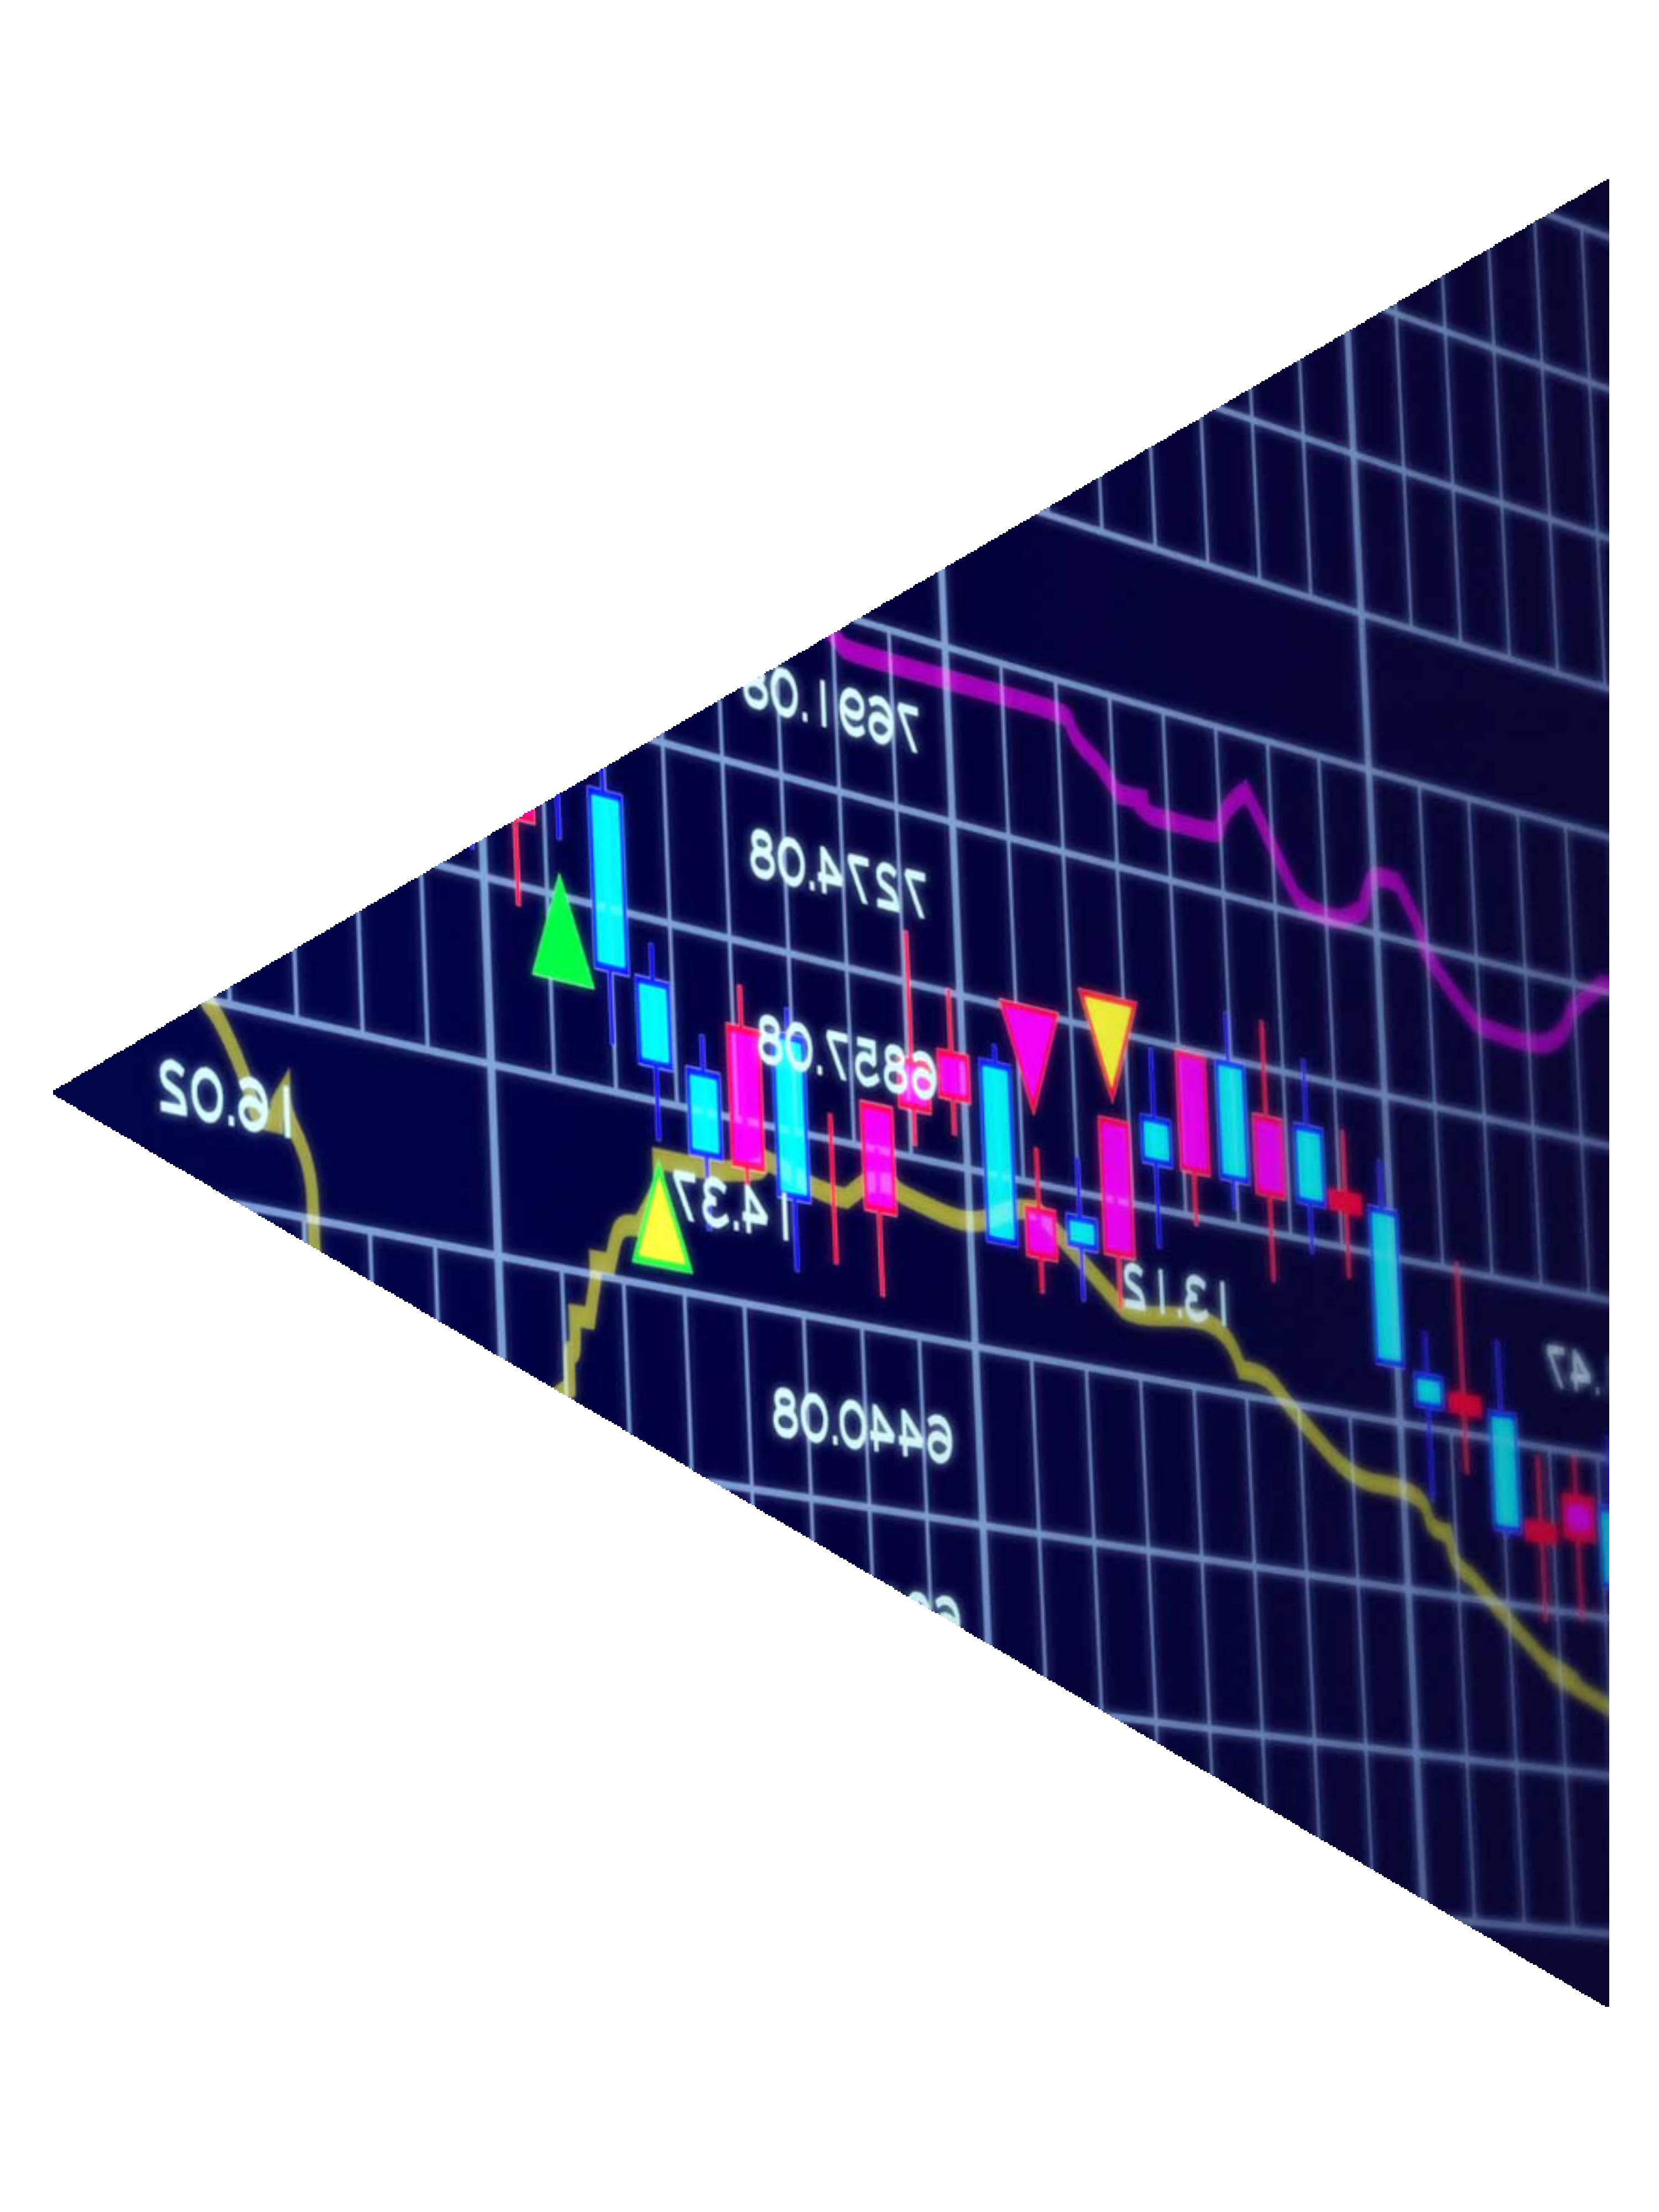
\includegraphics[width=22cm]{triangle.png}};
	\fill [jaune] (14,5) -- (2.5, 12) -- (20,25) -- (14, 20);
 \end{tikzpicture}}


\SetBgContents{\MyGraphicLogo}% Select included image

\SetBgPosition{current page.north west}% Select location
\SetBgOpacity{1.0}% Select opacity
\SetBgAngle{0.0}% Select roation of logo
\SetBgScale{1.0}% Select scale factor of logo

\usepackage{listings}
\usepackage{color}

\definecolor{mygreen}{rgb}{0,0.6,0}
\definecolor{mygray}{rgb}{0.5,0.5,0.5}
\definecolor{mymauve}{rgb}{0.58,0,0.82}

\lstset{ 
  backgroundcolor=\color{white},   % choose the background color; you must add \usepackage{color} or \usepackage{xcolor}; should come as last argument
  basicstyle=\footnotesize,        % the size of the fonts that are used for the code
  breakatwhitespace=false,         % sets if automatic breaks should only happen at whitespace
  breaklines=true,                 % sets automatic line breaking
  captionpos=b,                    % sets the caption-position to bottom
  commentstyle=\color{mygreen},    % comment style
  deletekeywords={...},            % if you want to delete keywords from the given language
  escapeinside={\%*}{*)},          % if you want to add LaTeX within your code
  extendedchars=true,              % lets you use non-ASCII characters; for 8-bits encodings only, does not work with UTF-8
  frame=single,	                   % adds a frame around the code
  keepspaces=true,                 % keeps spaces in text, useful for keeping indentation of code (possibly needs columns=flexible)
  keywordstyle=\color{blue},       % keyword style
  language=Octave,                 % the language of the code
  morekeywords={*,...},            % if you want to add more keywords to the set
  numbers=left,                    % where to put the line-numbers; possible values are (none, left, right)
  numbersep=5pt,                   % how far the line-numbers are from the code
  numberstyle=\tiny\color{mygray}, % the style that is used for the line-numbers
  rulecolor=\color{black},         % if not set, the frame-color may be changed on line-breaks within not-black text (e.g. comments (green here))
  showspaces=false,                % show spaces everywhere adding particular underscores; it overrides 'showstringspaces'
  showstringspaces=false,          % underline spaces within strings only
  showtabs=false,                  % show tabs within strings adding particular underscores
  stepnumber=2,                    % the step between two line-numbers. If it's 1, each line will be numbered
  stringstyle=\color{mymauve},     % string literal style
  tabsize=2,	                   % sets default tabsize to 2 spaces
  title=\lstname                   % show the filename of files included with \lstinputlisting; also try caption instead of title
}


%%%%%%%%%%%%%%%%%%%%%%%%%%%%%%%%%%%%%%%%%%%%%%%%%%%%%%%%%%%%%%%%%%%%
%																																	   %
%																																	   %
%																																	   %
%										Informations générales sur le document															   %
%																																	   %
%																																	   %
%%%%%%%%%%%%%%%%%%%%%%%%%%%%%%%%%%%%%%%%%%%%%%%%%%%%%%%%%%%%%%%%%%%%

 \usepackage{fontspec}
  \usepackage[bold-style=upright]{unicode-math}
  \defaultfontfeatures{Scale=1}
  \setmainfont[Ligatures=TeX,Numbers=OldStyle]{Lucida Bright OT}
  \setmathfont[RawFeature=+ss04]{Lucida Bright Math OT}
  \setsansfont[Scale=1.0,Numbers=OldStyle]{Myriad Pro}
  \newfontfamily\fullcaps[Letters=Uppercase,Numbers=Uppercase]{Myriad Pro}
  \usepackage[babel=true]{microtype}
  \usepackage{icomma}
  \usepackage{subcaption} 
  
  
  
  
  
  
  
  
  
  
  
\title{Greeks}
\author{Maxence COUPET - \href{mailto:maxence.coupet@gmail.com}{maxence.coupet@gmail.com}}
\date{March 2018}



\MHInternalSyntaxOn
\MH_set_boolean_T:n {outer_mult}
\MHInternalSyntaxOff

\newenvironment{nalign}{
    \begin{equation}
    \begin{aligned}
}{
    \end{aligned}
    \end{equation}
    \ignorespacesafterend
}
%%%%%%%%%%%%%%%%%%%%%%%%%%%%%%%%%%%%%%%%%%%%%%%%%%%%%%%%%%%%%%%%%%%%
%																																	   %
%																																	   %
%																																	   %
%												Mis en page du document																   %
%																																	   %
%																																	   %
%%%%%%%%%%%%%%%%%%%%%%%%%%%%%%%%%%%%%%%%%%%%%%%%%%%%%%%%%%%%%%%%%%%%


\begin{document}
	\selectlanguage{french}
	% page de garde
	\pagenumbering{gobble}
	\maketitle
	\newpage
	% début du rapport
	
	
	


\newcommand{\MyGraphicLog}{% For imported graphic logo
\begin{tikzpicture}[remember picture,overlay,yshift=-15cm, xshift=10.5cm]
\definecolor{jaune}{RGB}{16, 52, 78};
\fill[jaune] (-11, -16) -- (13, -16) -- (13, -12.1) -- (-11, -12.1);
 \end{tikzpicture}}


\SetBgContents{\MyGraphicLog}% Select included image


\SetBgPosition{current page.north west}% Select location
\SetBgOpacity{1.0}% Select opacity
\SetBgAngle{0.0}% Select roation of logo
\SetBgScale{1.0}% Select scale factor of logo

\pagestyle{fancy}
\renewcommand\headrulewidth{0pt}
\lhead{}\chead{}\rhead{}
\cfoot{\vspace*{6\baselineskip} \textcolor{white}{\thepage} \large}
	\newpage

	\pagenumbering{arabic}

%%%%%%%%%%%%%%%%%%%%%%%%%%%%%%%%%%%%%%%%%%%%%%%%%%%%%%%%%%%%%%%%%%%%
%																																	   %
%																																	   %
%																																	   %
%								Début du document (commencez à taper votre texte ici)													   %
%																																	   %
%																																	   %
%%%%%%%%%%%%%%%%%%%%%%%%%%%%%%%%%%%%%%%%%%%%%%%%%%%%%%%%%%%%%%%%%%%%

	Before we start with the computation of the several greeks, it is important to recal the Black-Scholes fomula for an european call and an european put paying no dividend.
	Let $S_0$ be the underlying price at time $0$, let $r$ be the risk-free rate, let $\sigma$ be the volatility of the underlying, let $T$ be the maturity of the option and $K$ the strike price. We then have :
	$$call(K, T) = S_0 N(d_1) - Ke^{rT}N(d_2)$$
	$$put(K, T) =  Ke^{rT}N(-d_2) - S_0 N(-d_1)$$
	
	with :
	$$d_1=\frac{ln\left(\frac{S_0}{K}\right)+(r+\frac{\sigma^2}{2})T}{\sigma\sqrt{T}}$$
	$$d_2=d_1 - \sigma\sqrt{T}$$
	
	
	\begin{figure}[!h]
	\centering
	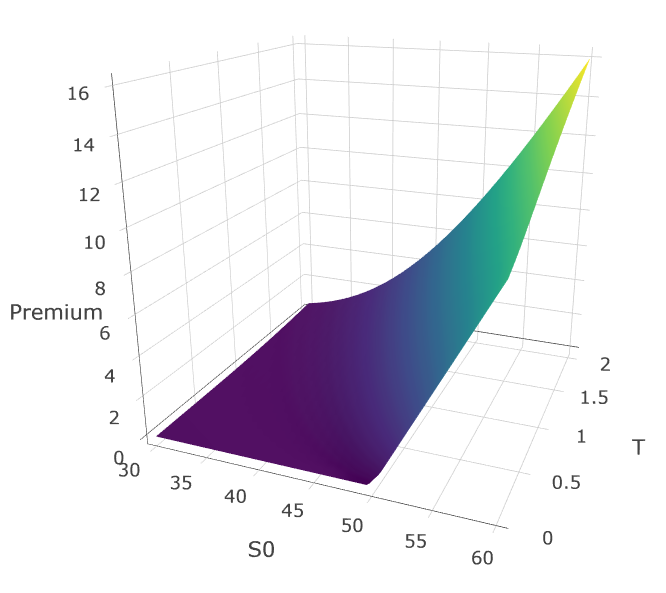
\includegraphics[width=\textwidth]{premium_call.png}
    \caption{Call premium}
    \label{fig:call_prem}
    \end{figure}
    
    \newpage
    \begin{figure}[!h]
	\centering
	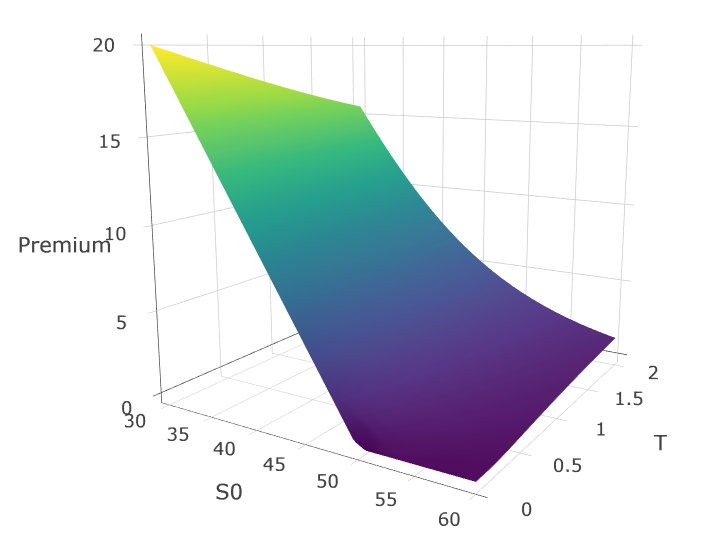
\includegraphics[width=\textwidth]{premium_put.png}
    \caption{Put premium}
    \label{fig:put_prem}
    \end{figure}
    
    
    Figures \ref{fig:call_prem} and \ref{fig:put_prem} show the premium of both call and put option for specific parameters ($K=50$, $\sigma=20\%$ and $r=10\%$) with different spot prices and time to maturity. It is quite interesting to know those shapes since the greeks are just derivatives with respect to different parameters. Thus, by observing the slope and convexity of those surface we can imagine the shape of the greeks. 
    
    Before we begin explaining each greek, one should be aware that knowing the 3D surface of the greeks, instead of just knowing a 2D representation is very useful in order to understand the greeks of combinaisons of options. A website is provided with this document (\href{https://maxencecoupet.shinyapps.io/options_greeks/}{link}) in order to allow everyone to manipulate the greeks in a 3D interractive environment. On this website you can rotate, zoom in and out on each greek and also change parameters of the options in order to better understand how each greek evolve with respect to different parameters (please note that site website is hosted on a free webservice provided by shinyapps.io and that connection could be lost with the server for no obvious reasons, just reload the page and continue what you were doing before being disconnected).
	
	\newpage
	\section{Greek letters}
	
	\subsection{Delta}
	
	The delta is the sensitivity of the option price with respect to changes in the underlying price. Therefore we can think of the delta as the slope of the price of the option with respect to the price of the underlying. One can show the following analytic formulas for calls and puts :
	$$ \Delta_{call}= \frac{\partial c}{\partial S} = N(d_1)$$
	$$ \Delta_{put}= \frac{\partial p}{\partial S} = N(d_1)-1$$
	
	An alternative way to define the delta, is the amount of shares needed in order to completely hedge a short position in the option with respect to changes in the underlying price. With a short position in a call, we will have losses if the price of the underlying increase. Therefore we are looking to take profit of such an increase by taking a position on the underlying (just in order to hedge the position), and we will buy shares (forward could be used too). Thus the delta will always be positive for a call. The same thinking could be made for a put, and show that the delta of a put is always negative since we sell shares in order to hedge our short position. 
	
	\begin{figure}[!h]
	\centering
	
	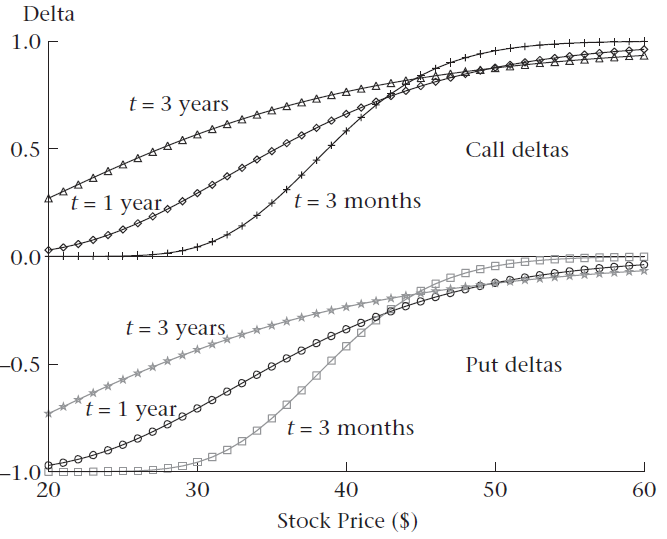
\includegraphics[width=0.7\textwidth]{delta_2d.png}
	
	\caption{Delta in 2D}
	\label{fig:delta2d}
	\end{figure}
	
	
	\begin{figure}[!h]
	\centering
	\caption{Delta surfaces}
  \begin{subfigure}[b]{0.45\textwidth}
    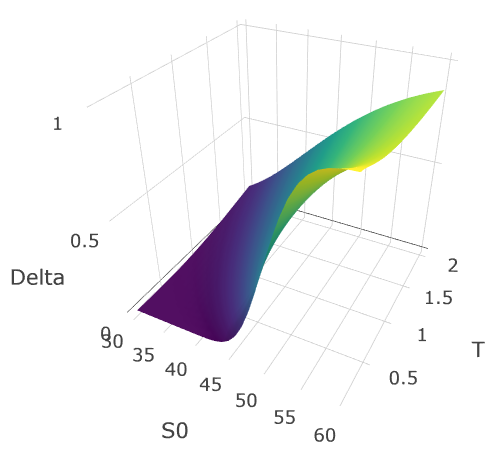
\includegraphics[width=\textwidth]{delta_call.png}
    \caption{Delta of a call}
    \label{fig:delta_call}
  \end{subfigure}
  %
  \begin{subfigure}[b]{0.45\textwidth}
    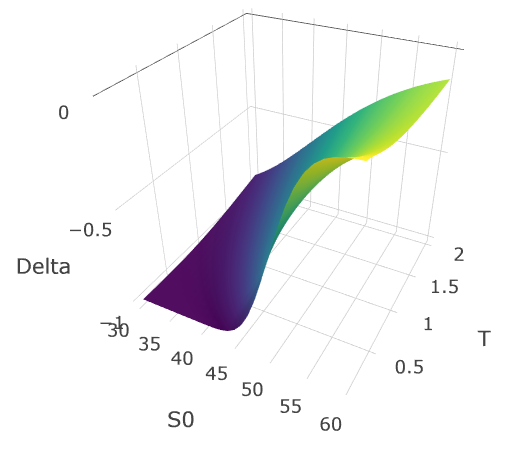
\includegraphics[width=\textwidth]{delta_put.png}
    \caption{delta of a put}
    \label{fig:delta_put}
  \end{subfigure}
\end{figure}

Figures \ref{fig:delta_call} and \ref{fig:delta_put} represent the delta for a call and a put in 3D and figure \ref{fig:delta2d} represent the same in 2D. We can see that the delta of a put is just a translation of the delta of a call. We have the two following properties :
$$ \Delta_{call} \in [0,1] \quad \quad \Delta_{put} \in [-1,0]$$

It is interesting to note that the delta is much steeper when the time to maturity is low, which means that when an option is at the money with a very short maturity, a little change in the underlying price would bring an import change in the delta (this is the gamma). Therefore performing delta hedging with an ATM option with short maturity is very challenging since the delta is constantly having important variations.

When explaining the delta we gave a solution for performing a delta hedging : taking positions in the underlying of the option with a size equal to the delta of the option (in \%). We have to keep in mind that a position is delta hedged only at one point in time, if the underlying price mooves, the position is no longer hedged because the value of the delta has changed, we therefore have to take a new position in the underlying in order to be delta hedged again. The process of constantly adjusting its hedging positions is reffered as \textbf{dynamic hedging} (opposed to static hedging when the trader only take one initial hedging position and does not touch it until maturity). Dynamic hedging could be very costly since it needs to make a lot of market orders (remember the commission fees and bid-ask spread), and finding the good period of refreshing for the hedge is the key factor in the cost of a dynamic hedging strategy. If the period is too short, the trader loose too much money in commision fees, but in the period in too long, then the position in the option is no longuer protected by the hedge. A solution would be to be gamma hedged : when one is gamma hedged, the delta will not change a lot and a higher period is possible.
\newpage
\subsection{Gamma}

	We saw that the delta could have important variation when the strike price is close to the spot price, therefore we need to use the second derivative of the option price with respect to the underlying price (or the derivative of the delta with respect to the underlying price) in order to characterize those variations of delta. One can show that calls and puts have the same gamma and it is given by the following analytic formula :
	$$ \Gamma= \frac{\partial^2 c}{\partial S^2} =\frac{\partial^2 p}{\partial S^2} = \frac{N'(d_1)}{S_0 \sigma \sqrt{T}}$$
	
	As we already discused in the section about delta, the delta only have important variation when the maturity is short and when the strike price is close to the spot price we could therefore anticipate the shape of the gamma in figure \ref{fig:gamma} and we can conclude that gamma hedging is only relevant for ATM options with relatively short maturity. 
	
	The gamma of a long position in a call or a put will always be non-negative and the gamma of a short position in a call or a put will always be negative.
	
	\begin{figure}[!h]
	\centering
	
	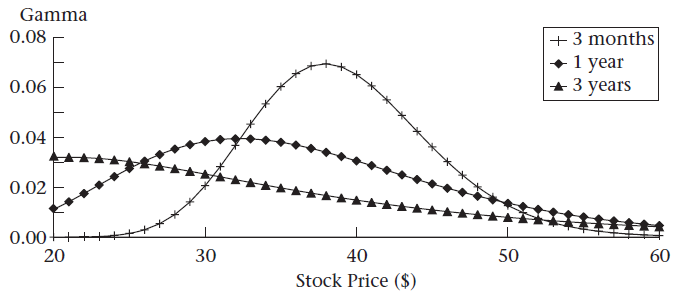
\includegraphics[width=0.7\textwidth]{gamma_2d.png}
	
	\caption{Gamma in 2D}
	\label{fig:gamma2d}
	\end{figure}
	
	\begin{figure}[!h]
	\centering
	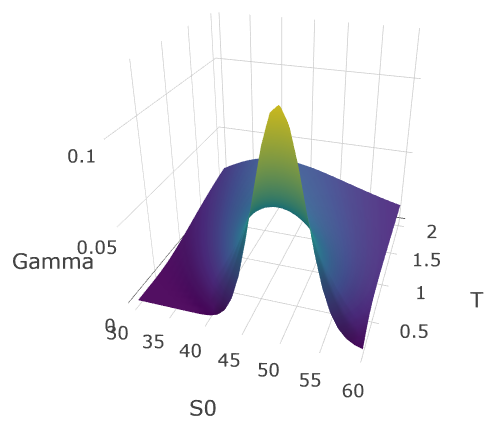
\includegraphics[width=0.7\textwidth]{gamma_call.png}
    \caption{Gamma surface of both call and put}
    \label{fig:gamma}
    \end{figure}
    
    One very important point with gamma is its relation with the theta of the option (discussed later in this document) : when the gamma of a position is positive, the theta will tend to be negative, which means that the position will tend to loose value when time passes except if there is an important moove (upward or downward) in the underlying price. The opposite also holds : when the gamma of a position is negative, the theta will tend to be positive, which means that the position will tend to gain value when time passes except if there is an important moove (upward or downward) in the underlying price.
    
    Since gamma is a second derivative of the price with respect to the underlying price, we have to find a financial product which has convexity with respect to the underlying price in order to hedge the gamma. The underlying is not enough because it has not convexity, in most cases we will use another option in order to gamma hedge. Let's consider that we have a short position on $n$ options (called option 1) with a gamma $\Gamma_1$ each, and that on the market, another option is available (called option 2) with a gamma $\Gamma_2$. In order to be gamma hedged, we will have to buy (since we are short option 1 and that the gamma of a short position is negative) $\frac{\Gamma_1}{\Gamma_2}n$ options 2. Our portfolio will then be gamma hedged but not delta neutral, we can make it delta neutral by taking the good position in the underlying (as explained in the previous section). The portfolio will then be delta-gamma hedged. Once again, keep in mind that as every greeks, the gamma may change over time, thus this hedge is only valid for a limited amount of time.
    
    For an ATM option, the gamma will be maximum for a short maturity, but for an OTM option, the gamma will be maximum for a long maturity. As we can see on figure \ref{fig:gamma}, the gamma is very dependant of the time to maturity so performing an exact gamma hedge could be of very little relevance with respect to time. It would make more sens to use a range for the gamma than an exact value.
    \newpage
    \subsection{Shadow gamma}
    Nassim Taleb is the one that popularized the notion of shadow gamma. The motivation for such a greek is that when we consider the gamma, we compute a partial derivative a thus suppose that all other parameters stay constant, which is not true in real life. The gamma is meant to measure the price sensibility of the option to big changes in the underlying price and it is easy to understand that an important mouvement in the underlying price will most likely happen with an important rise of volatility. Therefore considering that volatility stays constant while computing the gamme could lead to huge approximations and such a gamma would not be a good representation of the observed gamma. Such considerations for the variation of volatility for an important variation in the underlying price is motivated by what is called the smile of implied volatility.
    \begin{figure}[!h]
	\centering
	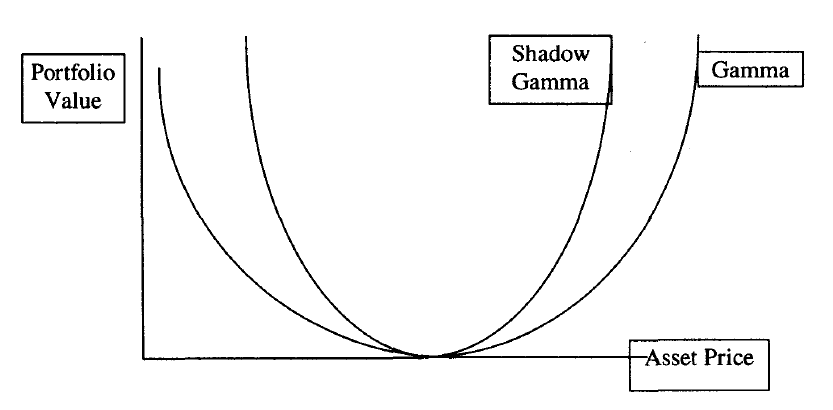
\includegraphics[width=0.7\textwidth]{shadow_gamma.png}
    \caption{Gamma and shadow gamma}
    \label{fig:shadow_gamma}
    \end{figure}
    
    The shadow gamma will then take into account the mouvement of the delta due to a mouvement in the underlying price and in the volatility. More advanced shadow gamma can take even more parameters such as the trader's expections with respect to changes in volatility and interest rates.
    A shadow greek is therefore a total derivative of the option price and not just a partial derivative.
    \newpage
    \subsection{Vega}
    
    The vega (vega is not a real greek letter by the way) represents the sensitivity of an option price to changes in volatility. By volatility we mean implied volatility of the option (see this link for more precisions about implied volatility : \href{https://www.investopedia.com/terms/i/iv.asp}{link}). An increase in volatility means that the underlying price is more likely to have important variations and thus finishing in the money. The vega will therefore be positive for a long position in a call or a put. Moreover, this increase in volatility will have a greater impact on greater maturities since the volatility will be higher for a longer period and could lead to an option very in the money. One can show that calls and puts have the same vega and it is given by the following analytic formula :
    $$\nu =\frac{\partial c}{\partial \sigma} =\frac{\partial p}{\partial \sigma}= S_0 \sqrt{T} N'(d_1)$$
    
    Figure \ref{fig:vega} show the vega surface for calls and puts. The important feature is to keep in minde that the vega is an increasing function of time to maturity.
    
    \begin{figure}[!h]
	\centering
	
	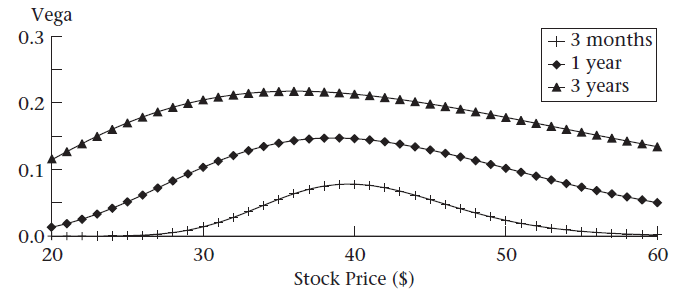
\includegraphics[width=0.7\textwidth]{vega_2d.png}
	
	\caption{Vega in 2D}
	\label{fig:vega2d}
	\end{figure}
    
    
    \begin{figure}[!h]
	\centering
	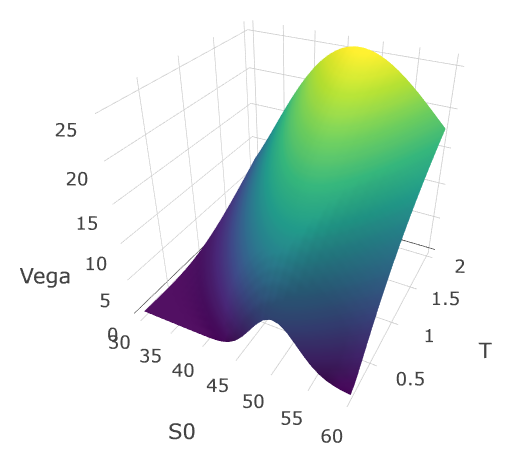
\includegraphics[width=0.7\textwidth]{vega.png}
    \caption{Vega surface of both call and put}
    \label{fig:vega}
    \end{figure}
    
    One could want to vega hedge his portfolio if it has an important maturity or if the strike price is close to the spot or even if the portfolio is made of a lot of positions in the same side (example : a straddle has an important vega since it is both long a call and a put). In order to vega hedge, we have to find a financial product that has sensibility to volatility. Since the underlying has no sensibility with respect to the volatility we will have to use another option in most cases. Let's consider a trader with a short position in $n$ options (called option 1) with a vega $\nu_1$ each, and that on the market another option is available (called option 2) with a vega $\nu_2$. In order to vega hedge the position, we will have to buy (since the vega of a short postion is negative) $\frac{\nu_1}{\nu_2}n$ options 2. The portfolio will then be vega hedge (again only for a limited period of time). One important point when vega hedging is not to hedge with short term options, since their vega will decrease very fast. Moreover, one does not want to void all his profit just in order to be vega hedged, therefore we should not use ATM options, which are very costly, to vega hedge. It would make more sens to hedge with OTM options because they are cheaper. Since we are short volotility we want to be protected against increase in volatility, if we use OTM options to vega hedge, a higher volatility would mean that our OTM options will tend to act as ATM options and thus have a higher vega, our hedge will therefore be better.  Finally, like when we were delta hedging, the vega hedging is only efficient locally, for small variations of the volatility. In order to be more accurate, we will have to consider the second derivative with respect to volatility : the volga.
    
    When an exotic product has a complexe sensitivity with respect to the volatility, the shape of vega could have different shapes along the term structure, those differents local shapes are call vega buckets.
    
    \newpage
    \subsection{Volga}
    The volga or vega-gamma (or Vomma) is the second derivative of the option price with respect to volatility (or the derivative of the vega with respect to volatility). It allow one to take in account the convexity of the option price with respect to volatility.
    
    For european options, only ITM and OTM options show convexity in volatility. Exotic options may have an important volga, like cliquet options or derivatives on volatility such as napoleons. The pricing of such products will thus have to take in account this convexity and the future cost of hedging this convexity.
    
    \newpage
    \subsection{Theta}
    
    The theta represents the sensibility of the option price to a variation in time. We already discussed the relationship between gamma and theta. One can show that the analytic formula for theta is given by :
    $$\theta_{call} = \frac{\partial c}{\partial t} = -\frac{S_0 \sigma N'(d_1)}{2\sqrt{T}} - rKe^{-rT}N(d_2)$$
    $$\theta_{put} = \frac{\partial p}{\partial t} = -\frac{S_0 \sigma N'(d_1)}{2\sqrt{T}} + rKe^{-rT}N(-d_2)$$
    
    Figures \ref{fig:theta_call} and \ref{fig:theta_put} show the theta for calls and puts. It is interesting to note that an deep-OTM put may have a positive theta, which means that a long position in a deep-OTM put has more value as time passes. But generally, the theta of a long position in both call or put is negative, which mean that all things being equal, the option losses value as time passes. One should be aware of this ''time decay'' when entering in a long postion. One should also note the non-symetric feature of the theta with respect to the underlying price.
    
    \begin{figure}[!h]
	\centering
	
	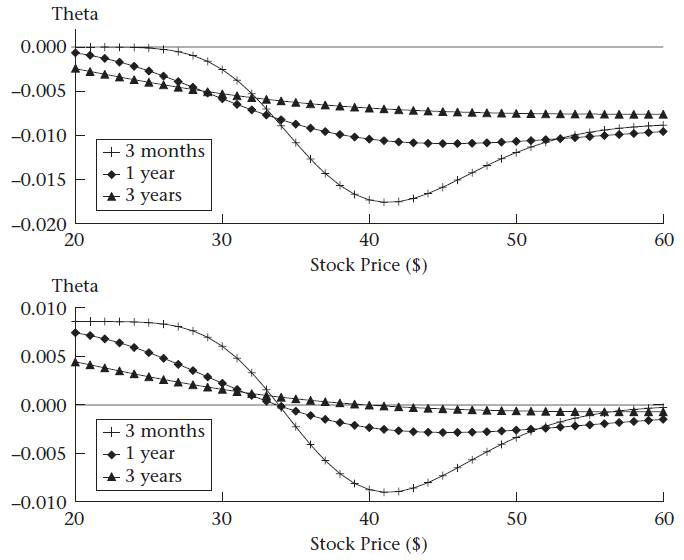
\includegraphics[width=0.7\textwidth]{theta_2d.png}
	
	\caption{Theta in 2D}
	\label{fig:theta2d}
	\end{figure}
    
    \begin{figure}
	\centering
	\caption{Theta surfaces}
  \begin{subfigure}[b]{0.45\textwidth}
    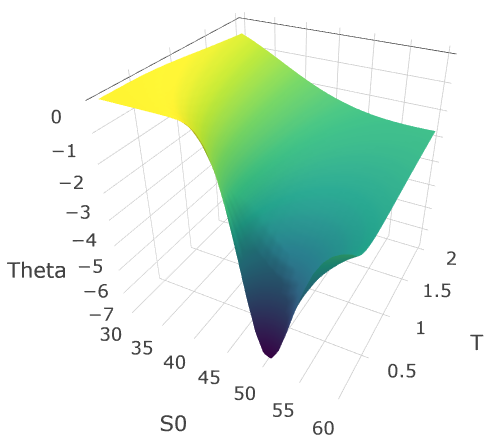
\includegraphics[width=\textwidth]{theta_call.png}
    \caption{Theta of a call}
    \label{fig:theta_call}
  \end{subfigure}
  %
  \begin{subfigure}[b]{0.45\textwidth}
    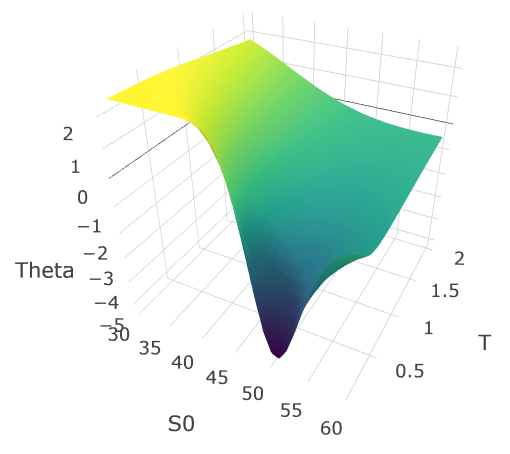
\includegraphics[width=\textwidth]{theta_put.png}
    \caption{Theta of a put}
    \label{fig:theta_put}
  \end{subfigure}
\end{figure}

\clearpage
    \subsection{Rho}
    
    The rho is the sensibility of the option price to variations in interest rates. A higher interest rates means that the expected value of the underlying price price will be higher (the drift of the stochastic process modeling the price is more important). Therefore a rise in interest rates is a good think for a long position in a call but a bad thing for a long position in a put and we can expect the rho of a call to be non-negative and the rho of a put to be negative.  One can show that the analytic formula for rho is given by :
    
    $$Rho_{call} = \frac{\partial c}{\partial r} = KTe^{-rT}N(d_2)$$
    $$Rho_{put} = \frac{\partial p}{\partial r} = -KTe^{-rT}N(-d_2)$$
    
    \begin{figure}[!h]
	\centering
	
	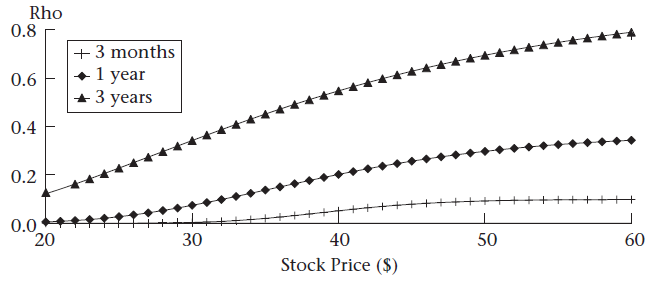
\includegraphics[width=0.7\textwidth]{rho_2d.png}
	
	\caption{Rho in 2D}
	\label{fig:rho2d}
	\end{figure}
    
    
    \begin{figure}[!h]
	\centering
	\caption{Rho surfaces}
  \begin{subfigure}[b]{0.45\textwidth}
    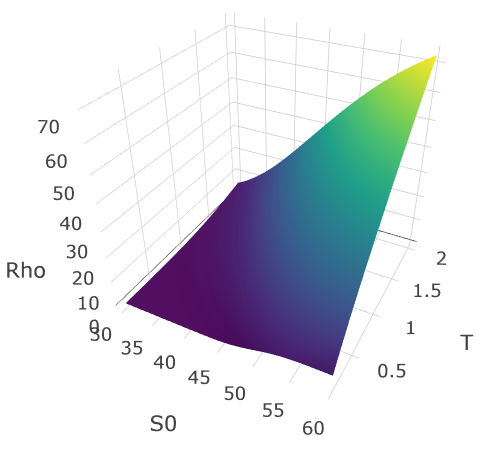
\includegraphics[width=\textwidth]{rho_call.png}
    \caption{Rho of a call}
    \label{fig:Rho_call}
  \end{subfigure}
  %
  \begin{subfigure}[b]{0.45\textwidth}
    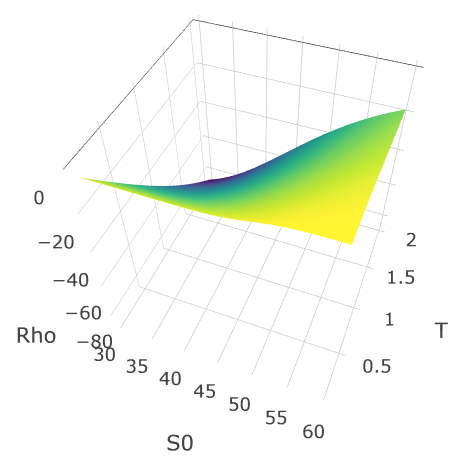
\includegraphics[width=\textwidth]{rho_put.png}
    \caption{Rho of a put}
    \label{fig:rho_put}
  \end{subfigure}
\end{figure}


\newpage
\subsection{Omega}
The delta give us an information about a rise of 1\$ in the underlying asset, but we do not have the information in percentages. This is the goal of omega, or option elasticity. The option elasticity is then defined by the delta of the option times the ratio between the underlying price and the option price $f$ :
$$\Omega = \Delta \frac{S}{f} $$

For a call, we will always have $\Omega \geq 1$ and for a put : $\Omega \leq 0$. Figure \ref{fig:omega}, shows the elasticity for a call option with parameters $K=40$, $\sigma = 0.3$ and $r=0.08$ :

\begin{figure}[!h]
	\centering
	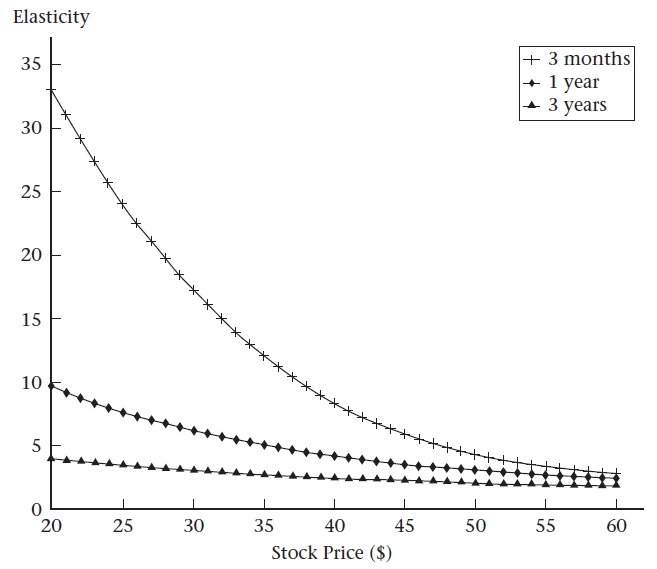
\includegraphics[width=0.6\textwidth]{omega.png}
    \caption{Omega of a call option}
    \label{fig:omega}
    \end{figure}
    
    It is important to understand that the Omega is a measure of the implicit leverage of the option, it is thus an interesting risk metric, in order to monitor the implicit leverage of the option over its life. 
    
    The more an option is OTM, the more important the implicite leverage will be. Thus for a call, the omega is an increasing function of the strike and for a put it is a decreasing function of the strike.
    
    The more an option is ITM, the more the option is likely to be exercized and thus the more the option looks like the underlying itself.  It is then logical to find that when an option tends to be deep ITM, the omega tends to be close to 1 since the underlying has an implicit leverage of 1.
    

\newpage
\section{Numerical methods for greeks}

While the Black-Scholes formula allow us to have an explicit formula for the greeks, when using a numerical method in order to price a more complicated derivative, we no longer have an explicit method for the greeks, we have to approximate. We will show how to do such a thing with the binomial tree model and with Monte-Carlo simulations. It is very important to understand the limitations of the approximation methods for the greeks. We will only present the finite differences method (see this document for other methods : \href{http://www.xaviermilhaud.fr/public/compteRendu-grecques.pdf}{link}) and an application for the delta, gamma and vega (other sensitivities can be obtain with similare calculations).

\subsection{Binomial tree}

When using the binomial tree method for pricing a derivative we both sample the time (generally we take $n$ steps) and the underlying price (the price can only go up or down, see figure \ref{fig:binom_tree}). Therefore computing the delta, the gamma and the theta is quite simple using finite differences method.

\begin{figure}[!h]
	\centering
	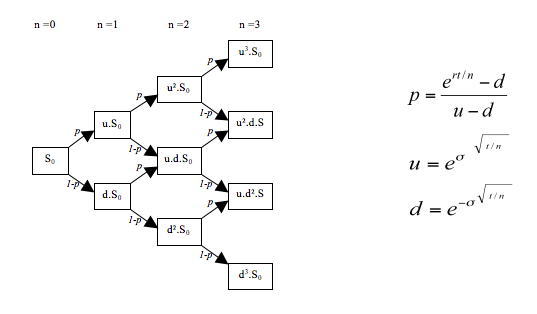
\includegraphics[width=\textwidth]{binom_tree.png}
    \caption{Binomial tree pricing method}
    \label{fig:binom_tree}
    \end{figure}
    
    Let $s_0$ be the initial stock price, let $u$ and $d$ be the up and down probability, let $\Delta t$ be the time period, let $c_u(t)$ and $c_d(t)$ be the prices of the call at time $t$ after an up and a down mouvement. 
    The finite difference to the first order state that :
    $$ \Delta \approx \frac{c_u(\Delta t) - c_d(\Delta t)}{S_0 u - S_0 d}$$
    
    In order to compute the gamma we need two value of the delta at time $2\Delta t$ :
    $$ \Gamma \approx  \frac{\frac{c_{uu}(2\Delta t) - c_{ud}(2\Delta t)}{S_0 u^2 - S_0} -  \frac{c_{ud}(2\Delta t) - c_{dd}(2\Delta t)}{S_0 - S_0 d^2}}{\frac{1}{2}(S_0 u^2 - S_0 d^2)}$$
    
    For the theta we also have all the information we need in the binomial tree : we only need two different prices of the option for the same underlying price but at different times. Thus if we take the option price at time $t=0$ and the option price at $t=2\Delta t$ for the path up-down (or down-up since we take a recombining tree), both options will have the same underlying price at different time, we then have :
    $$ \theta \approx  \frac{c_{ud}(2 \Delta t) - c(0)}{2 \Delta t}$$
    
    Computing the vega or the rho is a little bit more complicated since the information in the binomial tree is not enough to compute them. For the vega, we will have to compute another tree with a volatility $\sigma^* = \sigma + \Delta\sigma$. We will then have two different prices for two volatilities and the vega is given by :
    $$\nu \approx  \frac{c_{\sigma + \Delta \sigma}(0) - c_{\sigma}(0)}{\Delta \sigma}$$
    
    The same thinking could be used to compute the rho.
    
    We will test those approximations with a Python script (available in the \href{sec:binom}{annexe}). The application will be for an european call so that we could compare the approximation with the Black-Scholes theorical greeks. The results of the tests are available in the following table. We see that the approximation is quite good but as it would be predictible, the accuracy of the method decrease when we go to the second derivative, the error is bigger for the gamma.
    \newline
    
    
\begin{tabular}{|c|c|c|c|}
\hline
Greek & Theorical value & Binomial tree approximation & Error \\
\hline
$\Delta$ & 0.63683 & 0.63680 & 0.005 \% \\
\hline
$\Gamma$ & 0.01876 & 0.01877 & 0.085 \%\\
\hline
$\theta$ & -6.41403 & -6.41713 & 0.048 \% \\
\hline
$\nu$ & 37.52403 & 37.52435 & 0.001 \% \\
\hline
\end{tabular}

\newpage
\subsection{Monte-Carlo simulation}
When pricing with the Monte-Carlo method, the greeks can be obtain with the same pattern that the computation of the vega for the binomial tree method : we compute a first price, then change the good parameter and compute again the price. The finite diffrerence between the two price will be our sensitivity (see the Python code in \href{sec:mc}{annexe} for more details). Once again, we have to keep in mind that using this method with second or third derivative could lead to poor results. Results of this method are available in the following table.
\newline


\begin{tabular}{|c|c|c|c|}
\hline
Greek & Theorical value & Binomial tree approximation & Error \\
\hline
$\Delta$ & 0.63683 & 0.6377 & 0.137 \% \\
\hline
$\Gamma$ & 0.01876 & 0.0192 & 2.771 \%\\
\hline
$\nu$ & 37.52403 & 37.5792 & 0.147 \% \\
\hline
\end{tabular}
\newpage
\appendix
\section{Greeks computation with binomial tree method}
\label{sec:binom}
    \lstinputlisting[language=Python]{greeks_binomial_method.py}
    \newpage
\section{Greeks computation with Monte-Carlo method}
\label{sec:mc}
    \lstinputlisting[language=Python]{greeks_monte_carlo_method.py}
\end{document}